\documentclass[parskip=full]{scrartcl}

\pdfoutput=1

\title{Synthetic data generation: A literature review}

\author{%
	Joao Fonseca\(^{1*}\), Fernando Bacao\(^{1}\)
	\\
	\small{\(^{1}\)NOVA Information Management School, Universidade Nova de Lisboa}
	\\
	\small{*Corresponding Author}
	\\
	\\
	\small{Postal Address: NOVA Information Management School, Campus de
    Campolide, 1070--312 Lisboa, Portugal}
	\\
	\small{Telephone: +351 21 382 8610}
}

\usepackage{float}
\usepackage{graphicx}
\usepackage{geometry}
\geometry{%
	a4paper,
	left=18mm,
	right=18mm,
	top=18mm,
}
\usepackage{amsmath}
\usepackage{enumitem}
\usepackage[ruled,vlined]{algorithm2e}
\usepackage{booktabs}
\usepackage{pgfplotstable}
\pgfplotsset{compat=1.14}
\usepackage{longtable}
\usepackage{tabu}
\usepackage{hyperref}
\date{}

% use \citet for inline text references, \cite for normal citations
\usepackage[
    style=numeric,
    citestyle=numeric,
    sorting=none,
    natbib=true,
    backend=biber, 
    maxcitenames=1, 
    maxbibnames=99
]{biblatex}
\bibliography{references}
\usepackage{breakcites}

% Fix underfull hbox warnings in bilbliography
% Reference: https://tex.stackexchange.com/questions/10924/underfull-hbox-in-bibliography
\usepackage{etoolbox}
\apptocmd{\sloppy}{%
    \hbadness%
    10000\relax
}{}{}

% Fix overfull hbox warnings in bibliography
% Reference: https://tex.stackexchange.com/questions/171999/overfull-hbox-in-biblatex
\usepackage[T1]{fontenc}
\usepackage[final]{microtype}

% Highlight text: \hl
\usepackage{soul}

\definecolor{hypecol}{HTML}{0875b7}
\hypersetup{%
    colorlinks,
    linkcolor={hypecol},
    citecolor={hypecol},
    urlcolor={hypecol}
}

\begin{document}

\maketitle

\begin{abstract}

    The generation of synthetic data can be used for anonymization,
    regularization, oversampling, semi-supervised learning, self-supervised
    learning and various other tasks. The wide range of applications of these
    mechanisms motivated the development of new algorithms specialized in
    generating data for specific types of data and Machine Learning (ML)
    tasks. As a result, the analysis of the different types of generative
    models 

    % We provide a broad taxonomy to define data generation mechanisms

    % We provide an analysis on recommendations for the evaluation of the
    % quality of the synthetic data generated

\end{abstract}

\section{Introduction}~\label{sec:introduction}

Synthetic data is obtained from a generative process based on properties of
real data~\cite{assefa2020generating}. The generation of synthetic data is
essential for various domains and tasks. For example, synthetic data is used
as a form of regularizing neural networks (\textit{i.e.}, data augmentation)
\textbf{[CITATION]}. One form of anonymizing datasets is via the production of
synthetic observations (\textit{i.e.}, synthetic data generation)
\textbf{[CITATION]}. In settings where only a small portion of training data
is labeled, some techniques generate artificial data using both labeled and
unlabeled data with a modified loss function to train neural networks
(\textit{i.e.}, semi-supervised learning)~\cite{laine2017temporal}. In
imbalanced learning contexts, synthetic data can be used to balance the target
classes' frequencies and reinforce the learning of minority classes
(\textit{i.e.}, oversampling)~\cite{fonseca2021improving}. Some active
learning frameworks use data generation to improve the quality of data
selection and classifier training~\cite{kim2021lada}. Other techniques employ
data generation to produce deep neural networks without labeled data
(\textit{i.e.}, self-supervised learning)~\cite{grill2020bootstrap}.

The breadth of these techniques span multiple domains, such as facial
recognition~\cite{lv2017data}, Land Use/Land Cover mapping
\textbf{[CITATION]}, medical image processing \textbf{[CITATION]}, Natural
Language Processing~\cite{feng2021survey} or credit card default
prediction~\cite{alam2020investigation}. According to the domain and data
type, the data generation techniques used may vary significantly. Generally
speaking, some data generation mechanisms are specific to some domains, data
types or tasks. \hl{For example, \ldots}. Most, if not all, of these
techniques are applied on the input or output space.

However, there are various data generation techniques that are invariant to
the task or data types used. These techniques can be either applied in the
feature space~\cite{devries2017dataset} or in problems using tabular data.  On
the one hand, data generation in the feature space uses a generative model to
learn a manifold, lower-dimensional abstraction over the input
space~\cite{kingma2019introduction}, defined here as the feature space.  At
this level, any tabular data generation mechanism can be applied and
reconstructed into the input space if necessary. On the other hand, synthetic
data generation on tabular data can be applied to most problems. Although, the
choice of the generation mechanism is still dependant on (1) the importance of
the relationships found between the different features, (2) the ML task to be
developed and (3) the motivation for the generation of synthetic data. For
example, when generating data to address an imbalanced learning problem
(\textit{i.e.}, oversampling), the relationships between the different
features are not necessarily kept since the goal is to reinforce the learning
of the minority class by redefining an ML classifier's decision boundaries. If
the goal is to anonymize a dataset, perform some type of descriptive task, or
ensure a consistent model interpretability, these relationships need to be
kept.

Depending on the context, evaluating the quality of the generated data is a
complex task. For example, for image and time series data, perceptually small
changes in the original data can lead to large changes in the euclidean
distance~\cite{assefa2020generating, theis2016note}. The evaluation of
generative models typically account primarily for the performance in a
specific task, since good performance in one criterion does not imply good
performance on another~\cite{theis2016note}. However, in computationally
intensive tasks it is often impracticable to search for the optimal
configurations of generative models. To address this limitation, other
evaluation methods have been proposed to assist in this evaluation, which can
be distinguished into statistical divergence metrics and precision/recall
metrics~\cite{alaa2022faithful}. The relevant performance metrics found in the
literature are discussed in Section~\ref{sec:evaluating-synthetic-data}.

% Discuss Generative models -> Network based models

\subsection{Motivation and Contributions}

This literature review focuses on the generation mechanisms and generative
models underlying the different techniques where synthetic data is generated.
Specifically, we focus on techniques used in studies published since 2019. 
We focus on the ML perspective of synthetic data, as opposed to the practical
perspective. From a practical sense, synthetic data is used as a proxy of real
data. It is assumed to be inaccessible, essential and a secondary asset for
purposes such as education, software development, or systems
demonstrations~\cite{mannino2019real}. 

We focus on data generation techniques in the tabular and feature space
(\textit{i.e.}, embedded inputs) given its breadth in scope. Related
literature reviews are mostly focused on specific algorithmic applications,
with little to no emphasis on the core generative process. For this reason,
these techniques often appear ``sandboxed'', even though there is a
significant overlap between them. There are some related reviews to be
published since 2019. \citet{assefa2020generating} provides a general overview
of synthetic data generation for time series data anonymization in the finance
sector. \citet{hernandez2022synthetic} reviews data generation techniques for
tabular health records anonymization. \citet{raghunathan2021synthetic} reviews
synthetic data anonymization techniques that preserve the statistical
properties of a dataset. \citet{nalepa2019data} reviews data augmentation
techniques for brain-tumor segmentation. \citet{bayer2021survey} distinguishes
augmentation techniques for text classification into feature and data space,
while providing an extensive overview of augmentation methods within this
domain. However, the taxonomy proposed and feature space augmentation methods
are not necessarily specific to the domain. \citet{shorten2021text},
\citet{chen2021empirical}, \citet{feng2021survey} and \citet{liu2020survey}
also review data augmentation techniques for text data.
\citet{yi2019generative} review Generative Adversarial Network architectures
for medical imaging. \citet{wang2020survey} reviews face data augmentation
techniques. \citet{shorten2019survey} and \citet{khosla2020enhancing} discuss
techniques for image data augmentation. \citet{rashid2019times} review data
augmentation techniques for time-series data, specifically construction
equipment activity recognition. \citet{iwana2021empirical} and
\citet{wen2020time} also review time-series data augmentation techniques. The
analysis of related literature reviews \footnote{%
    Results obtained using Google Scholar, limited to articles published since
    2019, using the search query {\fontfamily{qcr}\selectfont (``synthetic
    data generation'' OR ``oversampling'' OR ``imbalanced learning'' OR ``data
    augmentation'') AND (``literature review'' OR ``survey'')}. Retrieved on
    August 11th, 2022.
} is shown in Table \hl{\textbf{XXXXX}}.


This literature review attempts to provide a
joint overview of the different data generation techniques, domains and ML
techniques where data generation is being used. 


The different taxonomies established are often specific to the technique
discussed. However, it is possible to establish a broader taxonomy without
giving up on specificity.

With this article, we aim to understand the current research gaps in the
different data mining techniques that involve synthetic data generation. We
compare the strengths and weaknesses of the models developed within each of
these fields. Finally, we identify possible future research directions to
address some of the limitations found.

Contributions of this paper are summarized below:

\begin{itemize}
    \item Bridge different ML concepts using synthetic data generation in its
        core \hl{(Algorithmic applications + Review of the State-of-the-art)}.
    \item List the different synthetic data generation/data augmentation
        taxonomies and characterize all relevant methods accordingly \hl{(Data
        augmentation taxonomy)}.
    \item Discuss the ML techniques in which synthetic data generation/data
        augmentation is used, beyond regularization and consolidate the
        current data generation mechanisms across the different techniques
        \hl{(Algorithmic Applications)}.
    \item Bring to light the key challenges of synthetic data generation and
        put forward possible research directions in the future.
\end{itemize}


% TODO: Develop research questions

\subsection{Paper Organization}

TODO TODO TODO TODO TODO TODO TODO TODO TODO TODO TODO TODO TODO TODO TODO
TODO TODO TODO TODO TODO TODO TODO TODO TODO TODO TODO TODO TODO TODO TODO
TODO TODO TODO TODO TODO TODO TODO TODO TODO TODO TODO TODO TODO TODO TODO
TODO TODO TODO TODO TODO TODO TODO TODO TODO TODO TODO TODO TODO TODO TODO
TODO TODO TODO TODO TODO TODO TODO TODO TODO TODO TODO TODO TODO TODO TODO
TODO TODO TODO TODO TODO TODO TODO TODO TODO TODO TODO TODO TODO TODO TODO

\section{Data Generation Taxonomy}

Image data augmentation taxonomy~\cite{khalifa2021comprehensive}

There is a distinction between semantic and traditional image data
augmentation~\cite{wang2021regularizing}, also discussed
in~\cite{shorten2019survey} 

Synthetic data generation for medical records
taxonomy~\cite{hernandez2022synthetic} which is incomplete



Data generation mechanisms can be characterized in 4 properties: Architecture,
Application level, Scope and Data space. The overall definition of the
proposed taxonomy is shown in Figure~\ref{fig:data-generation-taxonomy}.

\begin{enumerate}
    \item Level of application (External or Internal)
    \item Scope (Local or Global augmentation)
    \item Architectural approach (heuristic, network-based or others)
    \item Data space (Input, feature or output). Within feature and output: Domain
\end{enumerate}

\begin{figure}
	\centering
	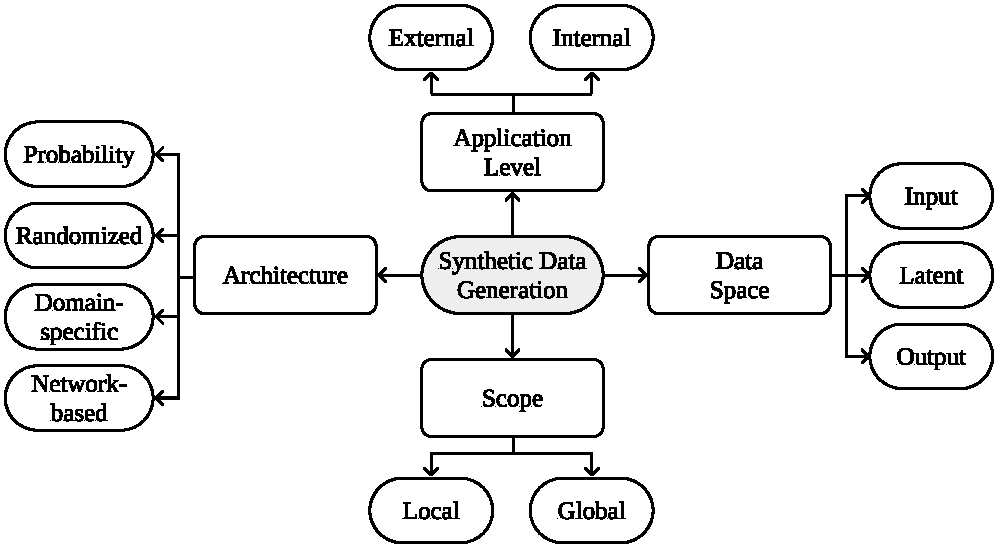
\includegraphics[width=.8\linewidth]{../analysis/data-generation-taxonomy}
    \caption{General taxonomy of data generation mechanisms proposed in this
        paper.
    }~\label{fig:data-generation-taxonomy}
\end{figure}


\section{Synthetic Data Generation}
% Feature level data augmentation

According to~\cite{assefa2020generating}. The generation of synthetic data
should aim to fulfil the conditions below:

\begin{itemize}
    \item Privacy preserving.
    \item Human readable.
    \item Compact.
\end{itemize}

\section{Data Generation Mechanisms}
% Review of the State-of-the-art of domain specific data generation

In this section, we describe some popular domain and data type-specific data
generation techniques. For each data type we include a table with related
literature reviews specific to different domains.

\subsection{Tabular}
% TODO: 
% - Table with literature review references 

\subsection{Time series}
% TODO: 
% - Table with literature review references 

Generative adversarial networks in time series 

\subsection{Image}
% TODO: 
% - Table with literature review references 

Image-specific data generation mechanisms can be further divided into
traditional and semantic techniques~\cite{wang2021regularizing}. Traditional
generation techniques comprise simple modifications such as translation,
cropping or random erasing~\cite{zhong2017random}. Semantic generation methods
involve more complex tasks, such changing colors of specific attributes,
backgrounds and visual angles \textbf{[CITATION]}. 
% Go back to explaining wang2021regularizing

% semantic generation technique
Data generation by modifying specific attributes in data points with known
perturbations~\cite{lv2017data}. For example, overlaying facial elements into
a picture containing a human face (\textit{e.g.}, adding sunglasses and
different hairstyles), introducing perturbations in facial landmarks,
different illumination and artificial misalignment are different approaches to
generate artificial observations for facial recognition.

% GANs
Generative Adversarial Networks in computer vision~\cite{wang2021generative}

% traditional
% - mixup

\subsection{Text}
% TODO: 
% - Table with literature review references 

NLP also benefit from data augmentation~\cite{feng2021survey}.

In NLP, there is the challenge of establishing universal rules for text
transformations to provide new linguistic patterns~\cite{bayer2022data}

https://github.com/styfeng/DataAug4NLP

\subsection{Graphs}

Superficial review on the topic here \cite{zhao2021data}

Another relevant paper \cite{zhou2020data}

\section{Algorithmic applications}

\subsection{Data Privacy}

% Introduce synthetic data generation
Synthetic data generation is a technique used to produce synthetic, anonymized
versions of datasets~\cite{dankar2021fake}. It is considered a good approach
to share sensitive data without compromising significantly a given data mining
task~\cite{taub2018differential, park2018data}. Traditional data anonymization
techniques, as well as federated learning are two other viable solutions for
privacy-preserving data publishing tasks, but contain
drawbacks~\cite{hernandez2022synthetic}. On the one hand, traditional data
anonymization requires domain knowledge, is labor intensive and remains
susceptible to disclosure~\cite{reiter2004new}. On the other hand, federated
learning is a technically complex task that consists on training ML
classifiers on edge devices and aggregating temporarily updated parameters on
a centralized server, instead of aggregating the training
data~\cite{yu2022survey}. Although it prevents sharing sensitive data, its
applicability is dependent on the task. Dataset anonymization via synthetic
data generation attempts to balance disclosure risk and data utility in the
final synthetic dataset. The goal is to ensure observations are not
identifiable and the relevant data mining tasks are not
compromised~\cite{singh2017aggregating, li2018privacy}.

The generation of synthetic datasets allow a more flexible approach to the
successful implementation of ML tasks. However,

Anonymizing data using synthetic data generation in the financial
sector~\cite{assefa2020generating}.

Guidelines for effective synthetic data generation~\cite{dankar2021fake}





\subsection{Regularization in Supervised Learning}

% Introduce data augmentation
The performance of Machine Learning models is highly dependent on the quality
of the training dataset used~\cite{Fenza2021, Halevy2009}. The presence of
imbalanced and/or small datasets, target labels incorrectly assigned, outliers
and high dimensional input spaces reduce the prospects of a successful machine
learning (ML) model implementation~\cite{Halevy2009, Domingos2012,
Salman2019}. In the case of deep learning, for example, these
models are often limited by a natural inclination to overfitting, label noise
memorization and catastrophic forgetting~\cite{Xie2021}. Regularization
methods are the typical approach to address these problems, but producing
robust ML solutions is still a challenge~\cite{Zhang2021}.

It is frequently assumed that the training data is sampled from a fixed data
source, it is balanced and does not contain label noise. Under these
conditions, the resulting ML classifier is expected to achieve good
generalization performance~\cite{benning2018modern}. Although, in practical
applications, this is rarely the case. When the training data is not
representative of the true population, or the model is over-parametrized, it
becomes particularly prone to overfitting~\cite{Bartlett2021}. Regularization
methods attempt to address these limitations. They can be divided into three
categories~\cite{santos2022avoiding}:

\begin{enumerate}
    \item Output level modifications. Transforms the labels in the training
        data.
    \item Algorithmic level modifications. Modifies the classifier's
        architecture, loss function or other components in the training
        procedure.
    \item Input level modifications. Modifies the training dataset by expanding it
        with synthetic data.
\end{enumerate}

The last approach, input level modifications, is known as data augmentation.
Data augmentation is used to increase the size and data variability of data in
a training dataset, by producing synthetic observations~\cite{Van2001,
Wong2016}. Since it is applied at the data level, it can be used for various
types of problems and classifiers~\cite{Behpour2019}. 

\subsection{Oversampling}

The original author of SMOTE recently published the paper ``Efficient Augmentation for Imbalanced Deep
Learning''~\cite{dablain2022efficient}

\subsection{Active Learning}

\subsection{Semi-supervised Learning}

\subsection{Self-supervised Learning}

\section{Evaluating the Quality of Synthetic Data
}~\label{sec:evaluating-synthetic-data}

The log-likelihood (and equivalently the Kullback-Leibler Divergence) is a
de-facto standard to train and evaluate generative
models~\cite{theis2016note}. Other common metrics include Parzen window
estimates, which~\citet{theis2016note} show that these metrics behave
independently and should generally be avoided. Therefore, it is necessary
to evaluate generative models with respect to the application these models are
being developed for.


The evaluation of generative models should quantify three key aspects of
synthetic data~\cite{alaa2022faithful}:

\begin{enumerate}
    \item Fidelity
    \item Diversity 
    \item Generalization
\end{enumerate}

The 3-dimensional metric proposed by~\citet{alaa2022faithful} quantifies these
aspects via the combination of three metrics ($\alpha$-Precision,
$\beta$-Recall and Authenticity) for various application domains.

\subsection{Statistical Divergence Metrics} 

\subsection{Precision/Recall Metrics}

\section{Discussion}

\subsection{Main Findings}

\subsubsection{RQ1: bla bla bla}

\subsubsection{RQ2: bla bla bla}

\subsubsection{RQ3: bla bla bla}

\subsection{Limitations}

Research across the different applications appears to be sandboxed even though
all techniques integrate synthetic data in its core.

% data privacy
The evaluation of anonymization techniques lack standardized, objective and
reliable performance metrics and benchmark datasets to allow an easier
comparison across classifiers to evaluate key aspects of data anonymization
(resemblance, utility, privacy and performance). These datasets should contain
mixed data types (\textit{i.e.}, a combination of categorical, ordinal,
continuous and discrete features) and the metrics should evaluate the
performance of different data mining tasks along with the anonymization
reliability.

% Regularization in supervised learning
Unlike with data privacy solutions, data augmentation techniques generally do
not consider the similarity/dissimilarity of synthetic data.

There is not a clear understanding of what types of data augmentation methods
are more appropriate according to different model architectures, ML tasks or
domains and the reason why they work better or worse depending on the task. 

% oversampling
There is a lack of research on oversampling solutions to generate synthetic
data with mixed data types and datasets with exclusively non metric features.

% Lack of methods adapted to use categorical features for tabular data

% Active Learning

% Semi-supervised Learning

% Self-supervised Learning
There is no clear understanding of the most appropriate data augmentation
techniques used to train self-supervised models and how their behavior and
performance varies according to the data generation method used.

% Societal challenges raised by data generation (?)
% Systematic bias

oversampling does not seem to be a relevant source of bias in behavioral
research and does not appear to have an appreciably different effect on
results for directly versus indirectly oversampled
variables~\cite{hauner2014latent}

% Maybe discuss adversarial attacks?

\subsection{Research directions}

% similarities between mixup and SMOTE, and an intermediate solution that can
% be further explored to use the mixup approach on tabular data
% (Geometric-SMOTE selection mechanism)

Quantifying the quality of the generated data:

\begin{enumerate}
    \item Realistic
    \item Similarity
    \item Usefulness (determine purpose and relevant performance metric)
    \item Understand the relationship between the 3 factors
\end{enumerate}

\section{Conclusions}

\printbibliography
\end{document}
